\RequirePackage[l2tabu, orthodox]{nag}
\RequirePackage{silence}
\documentclass[french,english]{beamer}
\input{preamble/packages}
\input{preamble/math_basics}
\input{preamble/math_mine}
\input{preamble/redac}
\input{preamble/draw}
\input{preamble/acronyms}

\title[Automatic argumentation]{Towards automatic argumentation about voting rules}
\subject{Social choice}
\keywords{empirical, theorem proving, automatic proofs}
\author{Michael Kirsten \inst{1} \and \emph{Olivier Cailloux} \inst{2}}
\institute[KIT, LAMSADE]{\inst{1} Dept. of Informatics, Karlsruhe Institute of Technology (KIT) \and \inst{2} LAMSADE, Université Paris-Dauphine}
\date{\formatdate{3}{7}{2018}}

\begin{document}
\begin{frame}[plain]
	\tikz[remember picture,overlay]{
		\path (current page.south west) node[anchor=south west, inner sep=0] {
			\includegraphics[height=1cm]{LAMSADE95.jpg}
		};
		\path (current page.south) ++ (0, 1mm) node[anchor=south, inner sep=0] {
			\includegraphics[height=9mm]{Dauphine.jpg}
		};
		\path (current page.south east) node[anchor=south east, inner sep=0] {
			\includegraphics[height=1cm]{PSL.png}
		};
		\path (current page.south) ++ (0, 4em) node[anchor=south, inner sep=0] {
			\scriptsize\url{https://github.com/oliviercailloux/voting-rule-argumentation-pres}
		};
	}
	\titlepage
\end{frame}
\addtocounter{framenumber}{-1}

\begin{frame}
	\frametitle{Introduction}
	\begin{block}{Context}
	\begin{itemize}
		\item Voting rule: a systematic way of aggregating different opinions and decide
		\item Multiple reasonable ways of doing this
		\item Different voting rules have different interesting properties
		\item None satisfy all desirable properties
	\end{itemize}
	\end{block}
	\begin{block}{Our goal}
		We want to easily communicate about strength and weaknesses of voting rules.
	\end{block}
\end{frame}

\begin{frame}
	\frametitle{Outline}
	\tableofcontents[hideallsubsections, sectionstyle=shaded/show]
\end{frame}

\AtBeginSection{
	\begin{frame}
		\frametitle{Outline}
		\tableofcontents[currentsection, hideallsubsections]
	\end{frame}
}

\section{Context}
\subsection{Introduction}
\begin{frame}[fragile]
	\frametitle{Voting rule}
	
	\begin{description}[Profile (on $A$)]
		\item[Alternatives] $\allalts = \set{a, b, c, d, \ldots}$; $\card{\allalts}=m$
		\item[Possible voters] $\allvoters = \set{1, 2, \ldots}$
		\item[Voters] $\emptyset \subset \voters \subseteq \allvoters$
%		\item[Linear orders on $A \subseteq \allalts$] $\linors$.
		\item[Profile] partial function $\prof$ from $\allvoters$ to linear orders on $\allalts$.
		\item[Voting rule] function $f$ mapping each $\prof$ to winners $\emptyset \subset A \subseteq \allalts$.
	\end{description}
	\vfill
	\begin{center}
		\begin{tikzpicture}
			\path node[profile matrix] (profile) {
				R_1&
				R_2
				\\
				| (profile11) | a&
				b
				\\
				b&
				a
				\\
				c&
				| (profile32) | c
				\\
			};
			\path ($(profile.south west)!.5!(profile.south east)$) ++ (0, -5mm) node {$\prof$};
			
			\path node[draw, rectangle, fit=(profile11) (profile32), outer xsep=2mm, outer ysep=1mm] (justprofile) {};
			\path (justprofile.east) ++ (2.5cm, 0) node[inner sep=0] (winners) {\mbox{} $A = \Set{a, b}$};
			\path[draw, ->] (justprofile.east) to[bend left=35] node[anchor=south] {$f$} (winners.west);

			\path[draw, decorate, decoration={brace, mirror}] (justprofile.south west) -- (justprofile.south east);
		\end{tikzpicture}
	\end{center}
\end{frame}

\begin{frame}[fragile]
	\frametitle{Example profile}
	\begin{equation}
		\begin{array}{lrrrrrr}
			&\multicolumn{6}{c}{\text{nb voters}}\\
		\cmidrule{2-7}
				&33	&16	&3	&8	&18	&22	\\
		\midrule
			1	&a	&b	&c	&c	&d	&e	\\
			2	&b	&d	&d	&e	&e	&c	\\
			3	&c	&c	&b	&b	&c	&b	\\
			4	&d	&e	&a	&d	&b	&d	\\
			5	&e	&a	&e	&a	&a	&a	\\
		\end{array}
	\end{equation}
	Who wins?\pause
	\begin{itemize}
		\item Most top-1: $a$
		\item $c$ is in the top 3 for everybody
		\item delete worst first, lowest nb of pref: $c$, $b$, $e$, $a$ ⇒ $d$
		\item delete worst first, from bottom: $a$, $e$, $d$, $b$ ⇒ $c$
		\item Borda: $b$
%		\item Condorcet: $c$
	\end{itemize}
\end{frame}

\subsection{Two voting rules}
\begin{frame}
	\frametitle{Borda}
	Given a profile $\prof$:
	\begin{itemize}
		\item score of $a \in \allalts$: number of alternatives it beats
		\item the highest scores win
	\end{itemize}
	
	\begin{equation}
		\prof =
		\begin{array}{rrrrr}
			a	&	a	&	a	&	b	&	b\\
			b	&	b	&	b	&	c	&	c\\
			c	&	c	&	c	&	a	&	a
		\end{array}
	\end{equation}
	\begin{itemize}
		\item score $a$ is\dots? \pause $2 + 2 + 2 = 6$
		\item score $b$ is $1 + 1 + 1 + 2 + 2 = 7$
		\item score $c$ is $1 + 1 = 2$
	\end{itemize}
	Winner: $b$.
\end{frame}

\begin{frame}
	\frametitle{Copeland}
	Given a profile $\prof$:
	\begin{itemize}
		\item score of $a \in \allalts$: number of alternatives against which it obtains a strict majority…
		\item … minus: number of alternatives that obtains a strict majority against $a$
		\item the highest scores win
	\end{itemize}
	
	
	\begin{equation}
		\prof =
		\begin{array}{rrrrr}
			a	&	a	&	a	&	b	&	b\\
			b	&	b	&	b	&	c	&	c\\
			c	&	c	&	c	&	a	&	a
		\end{array}
	\end{equation}
	\begin{itemize}
		\item score $a$ is\dots? \pause $\card{\set{b, c}} - \card{\emptyset} = 2$
		\item score $b$ is $\card{\set{c}} - \card{\set{a}} = 0$
		\item score $c$ is $\card{\emptyset} - \card{\set{a, b}} = -2$
	\end{itemize}
	Winner: $a$.
\end{frame}
	
\subsection{Axiomatic analysis}
\begin{frame}
	\frametitle{\subsecname}
	\begin{quote}
		Rather than dream up a multitude of arbitration schemes and determine whether or not each withstands the best of plausibility in a host of special cases, let us invert the procedure. Let us examine our subjective intuition of fairness and formulate this as a set of precise desiderata that any acceptable arbitration scheme must fulfil. Once these desiderata are formalized as axioms, then the problem is reduced to a mathematical investigation of the existence of and characterization of arbitration schemes which satisfy the axioms.
	\end{quote}
	\citet[p. 121]{luce_games_1957}\par
\end{frame}

\begin{frame}
	\frametitle{What’s an axiom?}
	\begin{itemize}
		\item An axiom (for us) is a principle
		\item Expressed formally
		\item That dictates some behavior of a voting rule
		\item In some conditions
		\item Usually seen as something to be satisfied
		\item Ideally, some union of some such axioms define exactly one rule
		\item Some axioms can be shown to be incompatible
	\end{itemize}
\end{frame}

\begin{frame}
	\frametitle{Unanimity}
	\begin{definition}[Unanimity]
		We may not select as winner someone who has some unanimously preferred alternative
	\end{definition}
	\begin{equation}
		\prof =
		\begin{array}{rrr}
			a	&	a	&	b\\
			b	&	b	&	c\\
			c	&	c	&	a
		\end{array}
	\end{equation}
	Constraint? \pause Do not take $c$ as $b$ is unanimously preferred to it.	\pause
	\begin{equation}
		\prof =
		\begin{array}{rrr}
			a	&	a	&	b\\
			b	&	c	&	c\\
			c	&	b	&	a
		\end{array}
	\end{equation}
	Constraint? \pause No constraint.
\end{frame}

\begin{frame}
	\frametitle{Condorcet’s principle}
	\begin{block}{Condorcet’s principle}
		We ought to take the Condorcet winner as sole winner if it exists.
		\begin{itemize}
			\item $a$ \emph{beats} $b$ iff more than half the voters prefer $a$ to $b$.
			\item $a$ is a \emph{Condorcet winner} iff $a$ beats every other alternatives.
		\end{itemize}
	\end{block}
	\vfill
	\begin{equation}
		\prof =
		\begin{array}{rrrrr}
			a	&	a	&	a	&	b	&	b\\
			b	&	b	&	b	&	c	&	c\\
			c	&	c	&	c	&	a	&	a
		\end{array}
	\end{equation}
	 Who wins? \pause $a$
\end{frame}

\begin{frame}
	\frametitle{Borda does not satisfy Condorcet}
	\begin{equation}
		\prof =
		\begin{array}{rrrrr}
			a	&	a	&	a	&	b	&	b\\
			b	&	b	&	b	&	c	&	c\\
			c	&	c	&	c	&	a	&	a
		\end{array}
	\end{equation}
	\begin{itemize}
		\item Borda winners? \pause $b$
		\item Condorcet winner? \pause $a$
	\end{itemize}
\end{frame}

\begin{frame}
	\frametitle{Cancellation}
	\begin{definition}[Cancellation]
		When all pairs of alternatives $(a, b)$ in a profile are such that $a$ is preferred to $b$ as many times as $b$ to $a$, we ought to select all winners as ex-æquo
	\end{definition}
	\begin{example}
		\begin{equation}
			f\left(%
			\begin{array}{rrrr}
				a&b&c&c\\
				b&a&a&b\\
				c&c&b&a\\
			\end{array}\right) = \allalts
		\end{equation}
	\end{example}
\end{frame}

\begin{frame}
	\frametitle{Reinforcement}
	\begin{definition}[Reinforcement]
		When joining two sets of voters, exactly those winners that each set accepts should be selected, if possible
	\end{definition}
	\begin{example}
		\begin{equation}
			\prof_1 =
			\begin{array}{cc}
				a&b\\
				b&a\\
				c&c\\
			\end{array},
			A_1 = \set{a, b},
			\prof_2 =
			\begin{array}{ccc}
				a&b&a\\
				b&a&c\\
				c&c&b\\
			\end{array},
			A_2 = \set{a},
		\end{equation}
		\begin{equation}
			\prof =
			\begin{array}{ccccc}
				a&b&a&b&a\\
				b&a&b&a&c\\
				c&c&c&c&b\\
			\end{array}.
			\text{ Winners? }
			\pause
			\set{a}
		\end{equation}
	\end{example}
\end{frame}

\subsection{Objective}
\begin{frame}
	\frametitle{Our objective}
	Produce automatically “arguments” of the kind: voting rule $f$ does not satisfy axiom $a$ on profile $R$
	\begin{itemize}
		\item To better understand their differences
		\item To help debate and choose a voting rule
		\item To investigate empirical attitudes towards given voting rules
	\end{itemize}
\end{frame}

\section{Approach}
\subsection{Overview}
\begin{frame}
	\frametitle{Overview}
	\begin{itemize}
		\item Given a voting rule $f$ and an axiom $a$
		\item $a$ indicates, given $\prof$ and winners $W$, if $(\prof, W)$ fails the axiom
	\end{itemize}
	\centering
	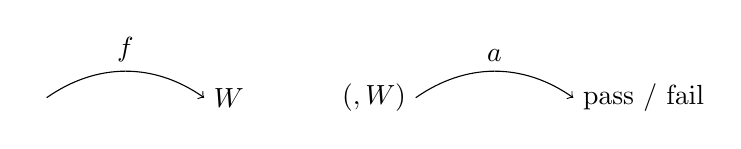
\begin{tikzpicture}
		\path node (R) {$\prof$};
		\path (R.east) ++ (2cm, 0) node[anchor=west] (W) {$W$};
		\path[draw, ->] (R.east) to[bend left=35] node[anchor=south] {$f$} (W.west);
		\path (W.east) ++ (1cm, 0) node[anchor=west] (RW) {$(\prof, W)$};
		\path (RW.east) ++ (2cm, 0) node[anchor=west] (out) {pass / fail};
		\path[draw, ->] (RW.east) to[bend left=35] node[anchor=south] {$a$} (out.west);
	\end{tikzpicture}
	\begin{block}{Objective}
		Find $\prof$ such that $(\prof, f(\prof))$ fails $a$
	\end{block}
	\begin{block}{Example}
		\begin{itemize}
			\item $f$ = Borda
			\item $a$ = Condorcet
			\item $f(\prof) = \set{b}$ (with $\prof$ used previously)
			\item $a(\prof, \set{b})$ fails
		\end{itemize}
	\end{block}
\end{frame}

\begin{frame}
	\frametitle{Overview}
	\begin{itemize}
		\item Given implementations \texttt{algo\_$f$} and \texttt{algo\_$a$}
	\end{itemize}
	\centering
	\begin{tikzpicture}
		\path node (R) {$\prof$};
		\path (R.east) ++ (2cm, 0) node[anchor=west] (W) {$W$};
		\path[draw, ->] (R.east) to[bend left=35] node[anchor=south] (af) {\texttt{algo\_$f$}} (W.west);
		\path (W.east) ++ (1cm, 0) node[anchor=west] (RW) {$(\prof, W)$};
		\path (RW.east) ++ (2cm, 0) node[anchor=west] (out) {pass / fail};
		\path[draw, ->] (RW.east) to[bend left=35] node[anchor=south] (aa) {\texttt{algo\_$a$}} (out.west);
		\onslide<2>{
			\path node[draw, color=red, rectangle, fit={(af) (W) (RW) (aa)}] (algo) {};
			\path (algo.south) node[anchor=north] {\color{red}{\texttt{algo}}};
		}
	\end{tikzpicture}
	\begin{itemize}
		\item We view it as a whole program \texttt{algo}
		\item We use SBMC, a software for checking properties of algorithms
		\item We let SBMC search for an input $\prof$ that fails \texttt{algo}
		\item Similar to searching for existence of a bug
	\end{itemize}
\end{frame}

\subsection{Software Bounded Model Checking}
\begin{frame}
	\frametitle{Checking properties}
%	\begin{lstlisting}
		assume(x > 0);\\
		i = 0;\\
		x0 = x;\\
		while (x < y) \{\\
		\hspace{2cm}	x += y;\\
		\hspace{2cm} i += 1;\\
		\}\\
		assert(x0+y*i >= x);
%		
%	\end{lstlisting}
	\begin{itemize}
		\item Given algorithm with parameters (example: $x$, $y$)
		\item Check that some property holds
		\item For all possible parameters
		\item … that satisfy given assumptions
		\item[⇒] search for $(x, y)$ that satisfy assumptions and fails assertion
	\end{itemize}
\end{frame}

\begin{frame}{Software Bounded Model Checking (SBMC)}
	\begin{block}{Specification}
		\begin{itemize}
			\item Properties specified using \texttt{assume} and \texttt{assert} statements
			\item A program \texttt{Prog} is \textbf{correct} iff:
			\[ \texttt{Prog} \wedge \bigwedge \texttt{assume} \Rightarrow \bigwedge \texttt{assert} \]
			\item \texttt{Prog} is automatically generated logical encoding of the program
		\end{itemize}
	\end{block}
	\begin{itemize}
		\item SBMC tool converts program into SAT
		\item Exhaustive check by unwinding the control flow graph
		\item Bounded in number of loop unwindings and recursions
		\item Special “unwinding assertion” claims added to check whether longer program paths may be possible
	\end{itemize}
\end{frame}

\begin{frame}
	\frametitle{Taking care of loops in SBMC}
	\texttt{while(x < y) x = x + y;}
	
	\begin{tikzpicture}
		\node (start) at (0,5.75) {};
		\node[ellipse, draw] (threea) at (-1.5,4) {\dots};
		\node[ellipse, draw] (threeb) at (1.5,4) {\texttt{x1 = x0 + y0;}};
		\node[ellipse, draw] (fivea) at (0, 2.5) {\texttt{x2 = x1 + y0;}};
		\node[ellipse, draw] (fiveb) at (3, 2.5) {\dots};
		\node[ellipse, draw] (seven) at (0, 1.5) {\dots};
		
		\path[-latex,draw] (start) -- (threea) node [midway, red, left] {\texttt{\textbf{!(x0 < y0)}}};
		\path[-latex,draw] (start) -- (threeb) node [midway,red, right] {\texttt{\textbf{x0 < y0}}};
		
		\path[-latex,draw] (threeb) -- (fivea) node [midway, red, left] {\texttt{\textbf{x1 < y0}}};
		\path[-latex,draw] (threeb) -- (fiveb) node [midway, red, right] {\texttt{\textbf{!(x1 < y0)}}};
		
		\path[-latex,draw] (fivea) -- (seven);
	\end{tikzpicture}
\end{frame}

\begin{frame}{Specifying and Verifying Properties in SBMC\hspace*{-1.8em}}
\begin{block}{Verification}
\begin{itemize}
\item Checking properties for programs generally undecidable
\item SBMC analyses only program runs up to \textbf{bounded} length
\item Property checking becomes decidable by logical encoding
\item Can be decided using SAT- or SMT-solver
\end{itemize}
\end{block}
\end{frame}

\section{Empirical results}
\subsection{Borda}
\begin{frame}
	\frametitle{Borda fails Condorcet}
	A minimal counter-example (found in less than one second):
	\begin{equation}
		\prof =
		\begin{array}{ccc}
			c	&	c	&	b\\
			b	&	b	&	a\\
			a	&	a	&	c
		\end{array}
	\end{equation}
	Borda rule elects $\{a,c\}$ instead of the Condorcet winner $c$
	
	The example can be easily inspected manually
\end{frame}

\begin{frame}
	\frametitle{Borda fails Weak Majority}
	A minimal counter-example in nb alts (< 1 sec):
	\begin{equation}
		\prof =
		\begin{array}{ccccc}
			a	&	a	&	a	&	b	&	b\\
			b	&	b	&	b	&	c	&	c\\
			c	&	c	&	c	&	a	&	a
		\end{array}
	\end{equation}
	Borda elects $b$ instead of the majority winner $a$.

	A minimal counter-example in nb voters (< 1 sec):
	\begin{equation}
		\prof =
		\begin{array}{ccc}
			d	&	d	&	c\\
			c	&	c	&	a\\
			a	&	b	&	b\\
			b	&	a	&	d
		\end{array}
	\end{equation}
	Borda elects $c$ instead of the majority winner $d$
\end{frame}

\subsection{Copeland}
\begin{frame}[fragile]
	\frametitle{Copeland fails Reinforcement}
	\begin{center}
	\begin{tikzpicture}[baseline]
    \begin{axis}[
    	title={Run-times for {\color{red}{2}}, {\color{green}{3}}, {\color{blue}{4}} and {\color{brown}{5}}
    	alternatives in seconds.},
    	height=0.8*\textheight,
    	xlabel={Voters},
    	ylabel={Run-time [minutes]},
    	xmin=2,xmax=10,
    	ymin=0,ymax=1800,
    	xtick={0,1,2,3,4,5,6,7,8,9,10},
    	xlabel near ticks,
    	ylabel near ticks,
     scaled y ticks={real:60},
        ytick scale label code/.code={},
   	ytick distance = 180
        ]
    	\addplot[red] table[x index=1,y index=2] {plots/copeland/reinforcement/cand_2.dat} node[pos=0.7,yshift=0.2cm,sloped] {2};
    	\addplot[green] table[x index=1,y index=2] {plots/copeland/reinforcement/cand_3.dat} node[pos=0.5,yshift=0.2cm,sloped] {3};
    	\addplot[blue] table[x index=1,y index=2] {plots/copeland/reinforcement/cand_4.dat} node[pos=0.6,yshift=0.2cm,sloped] {4};
    	\addplot[brown] table[x index=1,y index=2] {plots/copeland/reinforcement/cand_5.dat} node[pos=0.3,yshift=0.2cm,sloped] {5};
        \addplot[green, mark=*, only marks] table[x index=1,y index=2] {plots/copeland/reinforcement/cand_3_cexp.dat};
    	\addplot[blue, mark=*, only marks] table[x index=1,y index=2] {plots/copeland/reinforcement/cand_4_cexp.dat};
    	\addplot[brown, mark=*, only marks] table[x index=1,y index=2] {plots/copeland/reinforcement/cand_5_cexp.dat};
    \end{axis}
\end{tikzpicture}
	\end{center}
\end{frame}

\begin{frame}
	\frametitle{Copeland fails Reinforcement}
	A minimal counter-example (found in 32 seconds):
	\begin{equation}
		\prof_1 =
		\begin{array}{cc}
			b	&	a\\
			a	&	c\\
			c	&	b
		\end{array},
		\hspace{1em}
		\prof_2 =
		\begin{array}{cc}
			a	&	b\\
			b	&	a\\
			c	&	c
		\end{array}
	\end{equation}
	\begin{itemize}
		\item Elected for $\prof_1$ and $\prof_2$: $a$ and $\{a,b\}$ respectively.
		\item For the joined profile $\prof_1 \cup \prof_2$, Copeland elects $\{a,b\}$ instead of $a$.
	\end{itemize}
\end{frame}

\begin{frame}[plain]
	\addtocounter{framenumber}{-1}
	\begin{center}
		\huge
		\textit{Thank you for your attention!}
	\end{center}
\end{frame}

\appendix
\AtBeginSection{
}

\clearpage\pdfbookmark[2]{\refname}{\refname}
\begin{frame}[allowframebreaks]
	\frametitle{\refname}
 	\bibliography{zotero}
\end{frame}

\clearpage\pdfbookmark{License}{License}
\begin{frame}[plain]
	\frametitle{License}
	This presentation, and the associated \LaTeX{} code, are published under the \href{http://opensource.org/licenses/MIT}{MIT license}. Feel free to reuse (parts of) the presentation, under condition that you cite the author.
	
	Credits are to be given to \href{http://www.lamsade.dauphine.fr/~ocailloux/}{Olivier Cailloux}, Université Paris-Dauphine.
\end{frame}
\addtocounter{framenumber}{-1}
\end{document}

\begin{frame}
	\frametitle{\subsecname}
	\begin{itemize}
		\item 
	\end{itemize}
\end{frame}

